\section{Giới thiệu}
Bản thân thời gian vốn là dữ liệu một chiều, là trung tâm của việc phát hiện xu hướng, xác định các mẫu lặp lại và mối các mối quan hệ trong dữ liệu. Thời gian và dữ liệu hướng thời gian có những đặc điểm riêng biệt đáng để chúng ta nghiên cứu và xử lý như một kiểu dữ liệu riêng. Do tầm quan trọng của dữ liệu hướng thời gian, cấu trúc của nó đã được nghiên cứu trong nhiều ấn phẩm khoa học. 
\\ \\
Các ví dụ sau minh họa tầm quan trọng của thời gian. Hình (\ref{fig:f7.1}) thể hiện ba biểu diễn trực quan khác nhau của cùng một tập dữ liệu hướng thời gian, chứa số ca mắc cúm hàng ngày xảy ra ở miền bắc nước Đức trong khoảng thời gian ba năm. Dữ liệu thể hiện một mô hình tuần hoàn mạnh. Hình ngoài cùng bên trái sử dụng một biểu đồ đường đơn giản để trực quan hóa dữ liệu. Mặc dù thời gian cao điểm có thể được nhận ra dễ dàng, tuy nhiên khi kiểm tra biểu diễn này, hành vi theo chu kì của dữ liệu chỉ có thể được đoán và thật khó để phân biệt các chu kì mà trên thực tế có tồn tại. Ngược lại, hình ở giữa và hình bên phải biểu diễn một vòng tròn nhấn mạnh các đặc tính tuần hoàn của dữ liệu bằng cách sử dụng trục thời gian hình xoắn ốc. Với hình xoắn ốc bên trái, mô hình tuần hoàn không được phát hiện ra. Điều này là do độ dài chu kì được đặt là 24 ngày, không khớp với sự tuần hoàn của dữ liệu. Biểu diễn xoắn ốc bên phải được cài đặt với chu kì 28 ngày ngay lập tức tiết lộ sự tuần hoàn trong dữ liệu. Sự khác biệt có ý nghĩa thống kê về số trường hợp bệnh cúm được báo cáo lần lượt vào Chủ Nhật và Thứ Hai là khá rõ ràng. Chúng ta cũng sẽ thấy sự tuần hoàn này nếu đặt độ dài chu ki là 7 hoặc 14 ngày hoặc một bội (nhỏ) của 7 ngày.
\begin{figure}[H] % places figure environment here   
    \centering % Centers Graphic
    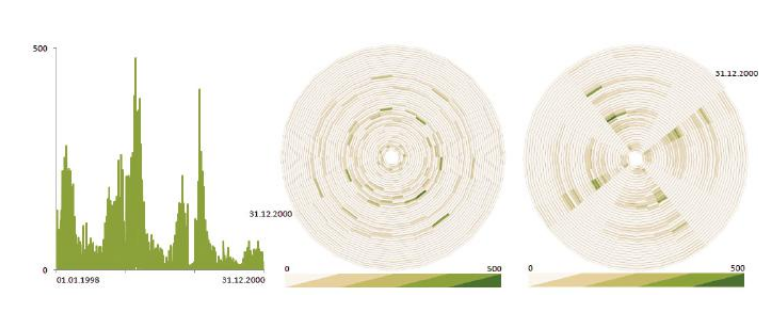
\includegraphics[width=0.8\textwidth]{assets/fg-1.png} 
    \caption{Đặc điểm của thời gian: tuyến tính so với biểu diễn theo chu kỳ của thời gian: những hiểu biết khác nhau
    có thể thu được từ các biểu diễn trực quan tùy thuộc vào việc tuyến tính hay tuần hoàn} % Creates caption underneath graph
    \label{fig:f7.1}
\end{figure}
Ví dụ này đã chứng minh một cách dễ hiểu rằng việc quan sát đặc tính thời gian có thể cải thiện đáng kể ý nghĩa của việc biểu diễn trực quan bằng hình ảnh. Do đó, điều quan trognj là phải chọn một biểu diễn trực quan phù hợp với đặc điểm của dữ liệu (theo chu kì trong trường hợp này) và tham số hóa phù hợp để có thể phát hiện các mẫu lặp lại ẩn trong dữ liệu. 
\\ \\
Trong phần tiếp theo, chúng ta sẽ nghiên cứu các đặc điểm của thời gian và dữ liệu hướng thời gian, thứ cần được xem xét và xử lý để lựa chọn kỹ thuật phù hợp.